\documentclass{beamer}
\usepackage{tikz}
\usetikzlibrary{arrows,shapes,matrix,positioning}

\begin{document}

\begin{frame}[fragile]{La matrice tableau di un PL in forma canonica}
\centering
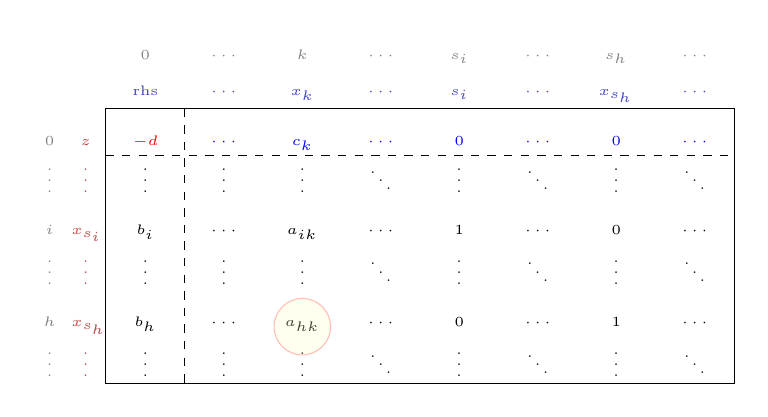
\begin{tikzpicture}
{\tiny
\node[%
  align=center,
  text width=3.5em,
  text height=5ex,
  row 1/.style={gray, text height=1em},
  row 2/.style={blue!50!gray, text height=1em},
  row 3/.style={blue},
  column 1/.style={gray,text width=1em},
  column 2/.style={red!50!gray,text width=1.5em},
  row 3 column 1/.style={gray},
  row 3 column 2/.style={red!50!gray},
  row 3 column 3/.style={red},
  matrix of math nodes] (M)
{%
% Indice delle righe (M-1)
~&~&0&\cdots&k&\cdots&s_i&\cdots&s_h&\cdots\\
% Intestazione delle colonne (M-2)
~ &~&  \mbox{rhs}& \cdots &  x_k &  \cdots & s_i & \cdots & x_{s_h} & \cdots \\
% Riga 0, fo e costi ridotti (M-3)
0 & z & -d & \cdots & c_k & \cdots & 0 & \cdots & 0 & \cdots\\
\vdots & \vdots &  \vdots &  \vdots &  \vdots &  \ddots &  \vdots &  \ddots &  \vdots &\ddots  \\
i& x_{s_i} & b_i & \cdots & a_{ik} &  \cdots & 1 & \cdots & 0 & \cdots\\
\vdots & \vdots &  \vdots &  \vdots &  \vdots &  \ddots &  \vdots &  \ddots &  \vdots &\ddots\\
h& x_{s_h} & b_h & \cdots & a_{hk} & \cdots & 0 & \cdots & {1} & \cdots\\
\vdots& \vdots &  \vdots &  \vdots &  \vdots &  \ddots &  \vdots &  \ddots &\vdots & \ddots\\
};

% riquadro
\draw(M-3-3.north west) -- (M-3-10.north east) -- (M-8-10.south east) -- (M-8-3.south west) -- cycle;

% separatore orizzontale
\draw[dashed] (M-4-3.north west) -- (M-4-10.north east);

% separatore verticale
\draw[dashed] (M-3-4.north west) -- (M-8-4.south west);

\draw[draw=red,fill=yellow!25,opacity=0.25] (M-7-5.base) circle (1.5 em);

}
\end{tikzpicture}
%sono fragile: lasciami uno spazio vuoto

\end{frame}
\end{document}
